
%----------------------------------------------------------------------------------------
%	PACKAGES AND DOCUMENT CONFIGURATIONS
%----------------------------------------------------------------------------------------

\documentclass[12pt,a4paper]{article}

\usepackage[version=3]{mhchem} % Package for chemical equation typesetting
\usepackage{siunitx} % Provides the \SI{}{} and \si{} command for typesetting SI units
\usepackage{graphicx} % Required for the inclusion of images
\usepackage{natbib} % Required to change bibliography style to APA
\usepackage{amsmath} % Required for some math elements 
\usepackage{geometry}
\usepackage{enumerate}
\usepackage{textcomp}
\usepackage{siunitx}
\usepackage{hhline}
\usepackage{caption}
\usepackage{booktabs}
\usepackage{multirow}
\usepackage{float}
\usepackage{longtable}

\renewcommand{\labelenumi}{\alph{enumi}.} % Make numbering in the enumerate environment by letter rather than number (e.g. section 6)
\geometry{left=2cm,right=2cm,top=3cm,bottom=3cm}

%\usepackage{times} % Uncomment to use the Times New Roman font

%----------------------------------------------------------------------------------------
%	DOCUMENT INFORMATION
%----------------------------------------------------------------------------------------


\begin{document}
\thispagestyle{empty}
\begin{center}

\Large{ \textsc{\newline\rule{14.3cm}{0.05em}\newline\\UM-SJTU Joint Institute\\Physics Laboratory\\(Vp141)\\}}
\rule{14.3cm}{0.05em}
\LARGE{\textsc{\newline\newline\newline\newline\newline\\
Laboratory Report\\}}
\Large{\textsc{  \\ Exercise 3  \\ Simple Harmonic Motion:
\\Oscillations in Mechanical Systems\\
} }

\end{center}

\begin{description}
    \item[] 
    \item[] 
    \item[] 
    \item[] 
    \item[] 
    \item[]
    \item[]
    \item[]
    \item[]\qquad \qquad Name: Han Yibei \qquad ID:519370910123   \qquad    Group:11        
    \item[]\qquad \qquad Date: \today
\end{description}

\newpage
\setcounter{page}{1}

%----------------------------------------------------------------------------------------
%	SECTION 1
%----------------------------------------------------------------------------------------

\section{Introduction}
The objective of this experiment is to study properties of a simple harmonic oscillation. We will first apply Hooke’s law to find out the spring constant. Then, we will do several control experiments on the air track to study the relationship between the oscillation period and the mass, the period and the amplitude, and the maximum speed and the amplitude.

\section{Theoratical background}
\subsection{Hooke's Law}
Within the elastic limit of deformation, the restoring force of the spring has the direction opposite to the deformation and its magnitude is directly proportional to the distance. Hooke’s Law can be expressed by:
\begin{equation}
    F_x=kx
\end{equation}
where k is the spring constant, $F_x$ is known as the restoring force and can be found using the Jolly balance.
\subsection{Equation of Motion of the Simple Harmonic Oscillator}
An object with mass M is placed on an air track which serves to eliminate the frictional force, as shown in Figure. 
\begin{figure}[H]
    \centering
        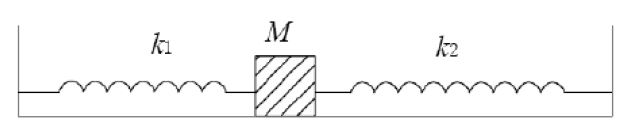
\includegraphics[width=13cm]{figure1.png}
        \caption{Mass-spring system}
\end{figure}
The two ends of the object are fixed to the air track using two springs whose spring constants are k1 and k2. Neglecting the masses of the springs and the damping and applying Newton’s second law, the equation of motion of the object is:s
\begin{equation}
    M\frac{d^2x}{dt^2}+(k_1+k_2)x=0\ \ \Rightarrow\ \ x(t)=A\cos{\omega_0t+\phi_0}
\end{equation}
where $\omega_0=\sqrt{(k_1+k_2)/M}$, which is the natural angular frequency of the oscillations and is determined by the parameters of the system itself. A is the amplitude and $\phi_0$ is the initial phase which is determined by initial conditions.\par 
The natural period of oscillation is:
\begin{equation}
    T=\frac{2\pi}{\omega_0}=2\pi\sqrt{\frac{M}{k_1+k_2}}\ \ \Rightarrow\ \     \frac{T^2}{m}=\frac{4\pi^2}{k_1+k_2}
\end{equation}

\subsection{Mass of the Spring}
When the mass of springs cannot be ignored, we consider the effective mass of the spring, which is 1/3 of the actual mass of the spring. The oscillator with object of mass M and spring of effective mass $m_0$ has the angular frequency:

\begin{equation}
    \omega_0=\sqrt{\frac{k_1+k_2}{M+m_0}}
\end{equation}

\subsection{Mechanical Energy in Harmonic Motion}
The elastic potential energy of the spring-mass system is $U=kx^2/2$ and the kinetic energy of it is $K=mv^2/2$.\par 
The speed of the mass is maximized at the equilibrium position x=0, where the total mechanical energy equals to maximum kinetic energy. At maximum displacement, the mass has no speed and has maximum potential energy as the total mechanical energy. Therefore, as there are only conservative forces, Kmax = Umax, and we get:
\begin{equation}
    k=\frac{mv^2_{max}}{A^2}
\end{equation}

Other things needed: $\Delta x=(x_{in}+x_{out})/2$, $v_{max}=\Delta x/\Delta t$. Where $x_{in}$ is the distance within the two legs of the U shape shutter and $x_{out}$ is the outer distance. $\Delta t$ is the time it takes to travel from one leg of the U shape shutter to the other, which is measured by the timer.


\section{Experimental setup}
The measurement equipment consists of: springs, Jolly balance, air track, electronic timer, electronic balance, and masses.

\subsection{Jolly balance}
The scale on the Jolly balance is used to measure the deformation of the spring, from which we can calculate the spring constant.
\begin{figure}[H]
    \centering
    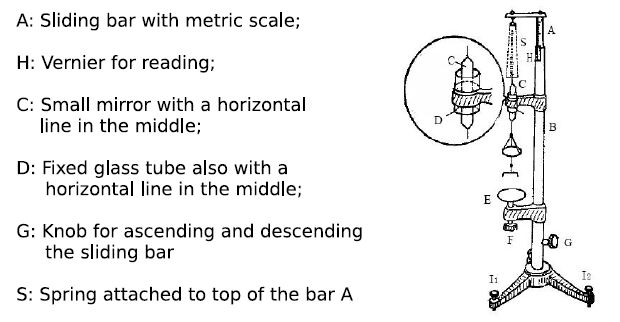
\includegraphics[width=12cm]{jollybalance.png}
    \caption{Jolly Balance}
    \label{jolly}
\end{figure}

First, put the initial 20g mass on the bottom end of the spring, read the scale L1. Then add mass m to it and read L2. The spring constant can be found as:
$$k=\frac{mg}{L2-L1}$$\par
Read the readings onlly if the three lines coincide: the line on the mirror, the line on the glass tude and its reflection in the mirror.

\subsection{Photoelectric Measuring System}
For period measurement, we use the I-shape shutter on the moving object to block the light emitted from the photoelectric gate. Each time the light is blocked, half a period is counted.\par 
For speed measurement, we use a U-shape shutter so that the light is blocked twice during a pass. The time interval ∆t is measured by the timer, and we use a caliper to measure the distance $x_{in}$ and $x_{out}$  to get $\Delta_x=\frac{1}{2}(x_{in}+x_{out})$. Therefore, the instantaneous speed can be expressed by $v=\frac{\Delta_x}{\Delta_t}$.

\begin{figure}[H]
    \centering
    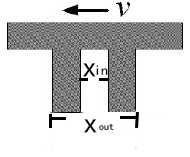
\includegraphics[width=5cm]{ushape.png}
    \caption{the U-shape shutter}
\end{figure}

\begin{figure}[H]
    \centering
    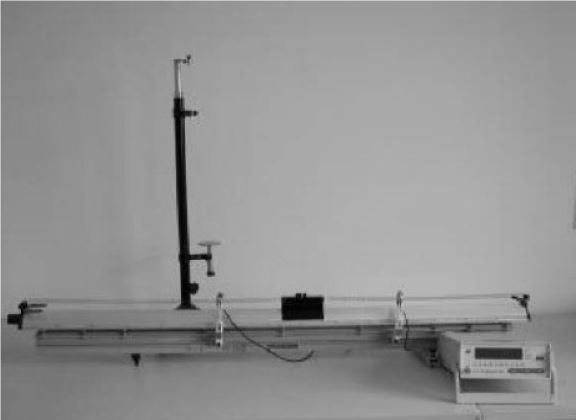
\includegraphics[width=12cm]{setup.png}
    \caption{the experimental setup}
\end{figure}

\subsection{Device information}

\begin{table}[H]
    \centering
    \begin{tabular}{ccc}
        \hline
    Apparatus & & Precision \\\hline  
    Jolly Balance & & 0.02[mm] \\ 
    Caliper & & 0.02[mm]  \\
    Electronic balance & & 0.01[g] \\
    \multirow{2}{*}{Photoelectric measuring system} & Mode $T$   & 0.0001[s]       \\
    & Mode $S_2$ & 0.00001[s]     \\
    Air track & & 0.1[cm]       \\\hline
    \end{tabular}
    \caption{Information of Each Measurement Device}
\end{table}

\section{Measurement}
\subsection{Spring Constant}
\begin{enumerate}[1.]
    \item Adjust the Jolly balance to be vertical, and add a 20g preload to the bottom end of the spring. (Fig.??j) Make sure the mirror can move freely.
    \item Adjust the position of the tube to set the initial position L0 within 5.0-10.0cm and record.
    \item Add mass m1 and record L1. 
    \item Keep adding masses in order and record 7 sets of positions in total. 
    \item Use the least square method to estimate the spring constant k1.
    \item Replace spring1 with spring2 and repeat the above steps to get spring constant k2.\item Remove the preload and repeat the measurement for springs1 and 2 connected in series and calculate k3. Compare k3 with theoretical value.
\end{enumerate}

\subsection{Relation Between the Oscillation Period T and the Mass of the Oscillator M}
\subsubsection{Adjustment of the air truck}
\begin{enumerate}[1.]
    \item Adjust the air track to be horizontal. 
    \item Turn on the air pump and check if there are any holes blocked.
    \item Place the cart on the track without initial velocity and adjust the single knob until the object moves slowly back and forth in both directions.
\end{enumerate}
Caution: Don’t place anything on the track when it’s off.

\subsubsection{Horizontal air track}
\begin{enumerate}[1.]
    \item Attach the I-shape shutter to the cart and attach springs to the sides of the cart to connect it to the air track. Make sure the photoelectric gate is at the equilibrium position.
    \item Add weight m1 and let the cart oscillate about the photoelectric gate. Use a pen to release the cart and ensure that the amplitude is about 5cm. Set the timer into ‘T’ mode and it will automatically record the time of 10 oscillation periods. Record both the total time and the mass of cart. 
    \item Add weights to the cart. Repeat step 2 and take the measurements for 5 times.
    \item Plot a graph to analyze the relation between T and M.  
\end{enumerate}

\subsubsection{inclined aire track}
\begin{enumerate}[1.]
    \item Place three plastic plates under one side of the air track. Repeat steps in 4.2.2.
    \item Add three plastic plates under that side and repeat steps in 4.2.2.
    \item Plot a graph to analyze the relation between T and M. 
\end{enumerate}

\subsection{Relation Between the Oscillation Period T and the Amplitude A}
\begin{enumerate}[1.]
    \item  Fix the mass of the cart and measure the period under 6 different values of the amplitude. The recommended amplitude is 5.0/10.0/…/30.0cm.
    \item linear fit to the data and analyze the relation between T and A based on the correlation coefficient $\gamma$.
\end{enumerate}

\subsection{ Relation Between the Maximum Speed and the Amplitude}
\begin{enumerate}[1.]
    \item   Use a caliper to measure $x_{out}$ and $x_{in}$ of the U-shape shutter. Calculate the distance $\Delta x=(x_{in}+x_{out})/2$.
    \item Replace the I-shape shutter with the U-shape shutter. Set the timer into ‘S2’mode.
    \item  Measure the maximum speed of the cart under 6 different values of amplitude. The recommended amplitude is 5.0/10.0/…/30.0cm. Record the second readings of the time interval only if the two subsequent readings show the same digits to the left of the decimal point.
    \item  Apply the data to calculate the spring constant k in Eq.6 and compare this result to that in 4.1.
\end{enumerate}

\subsection{Mass measurement}
\begin{enumerate}[1.]
    \item Adjust the electronic balance every time before you use it.
    \item First weigh the cart with the I-shape shutter, then the cart with the U-shape shutter. Then measure the mass of spring1 together with spring2.
    \item Record the data only after the circular symbol on the scales display disappears.
\end{enumerate}
%----------------------------------------------------------------------------------------
%	SECTION 6
%----------------------------------------------------------------------------------------

\section{Results}
\subsection{Measurement of the spring constant}

The acceleration due to gravity given by instructor is 9.794$m/s^2$, we use the formula w=mg to calculate the weight:
Take 1 as example, $w=mg=4.88\times 10^(-3)\times 9.794=0.0478\pm 9.794\times 10^(-5) N.$

\begin{center}
    \begin{figure}[H]
    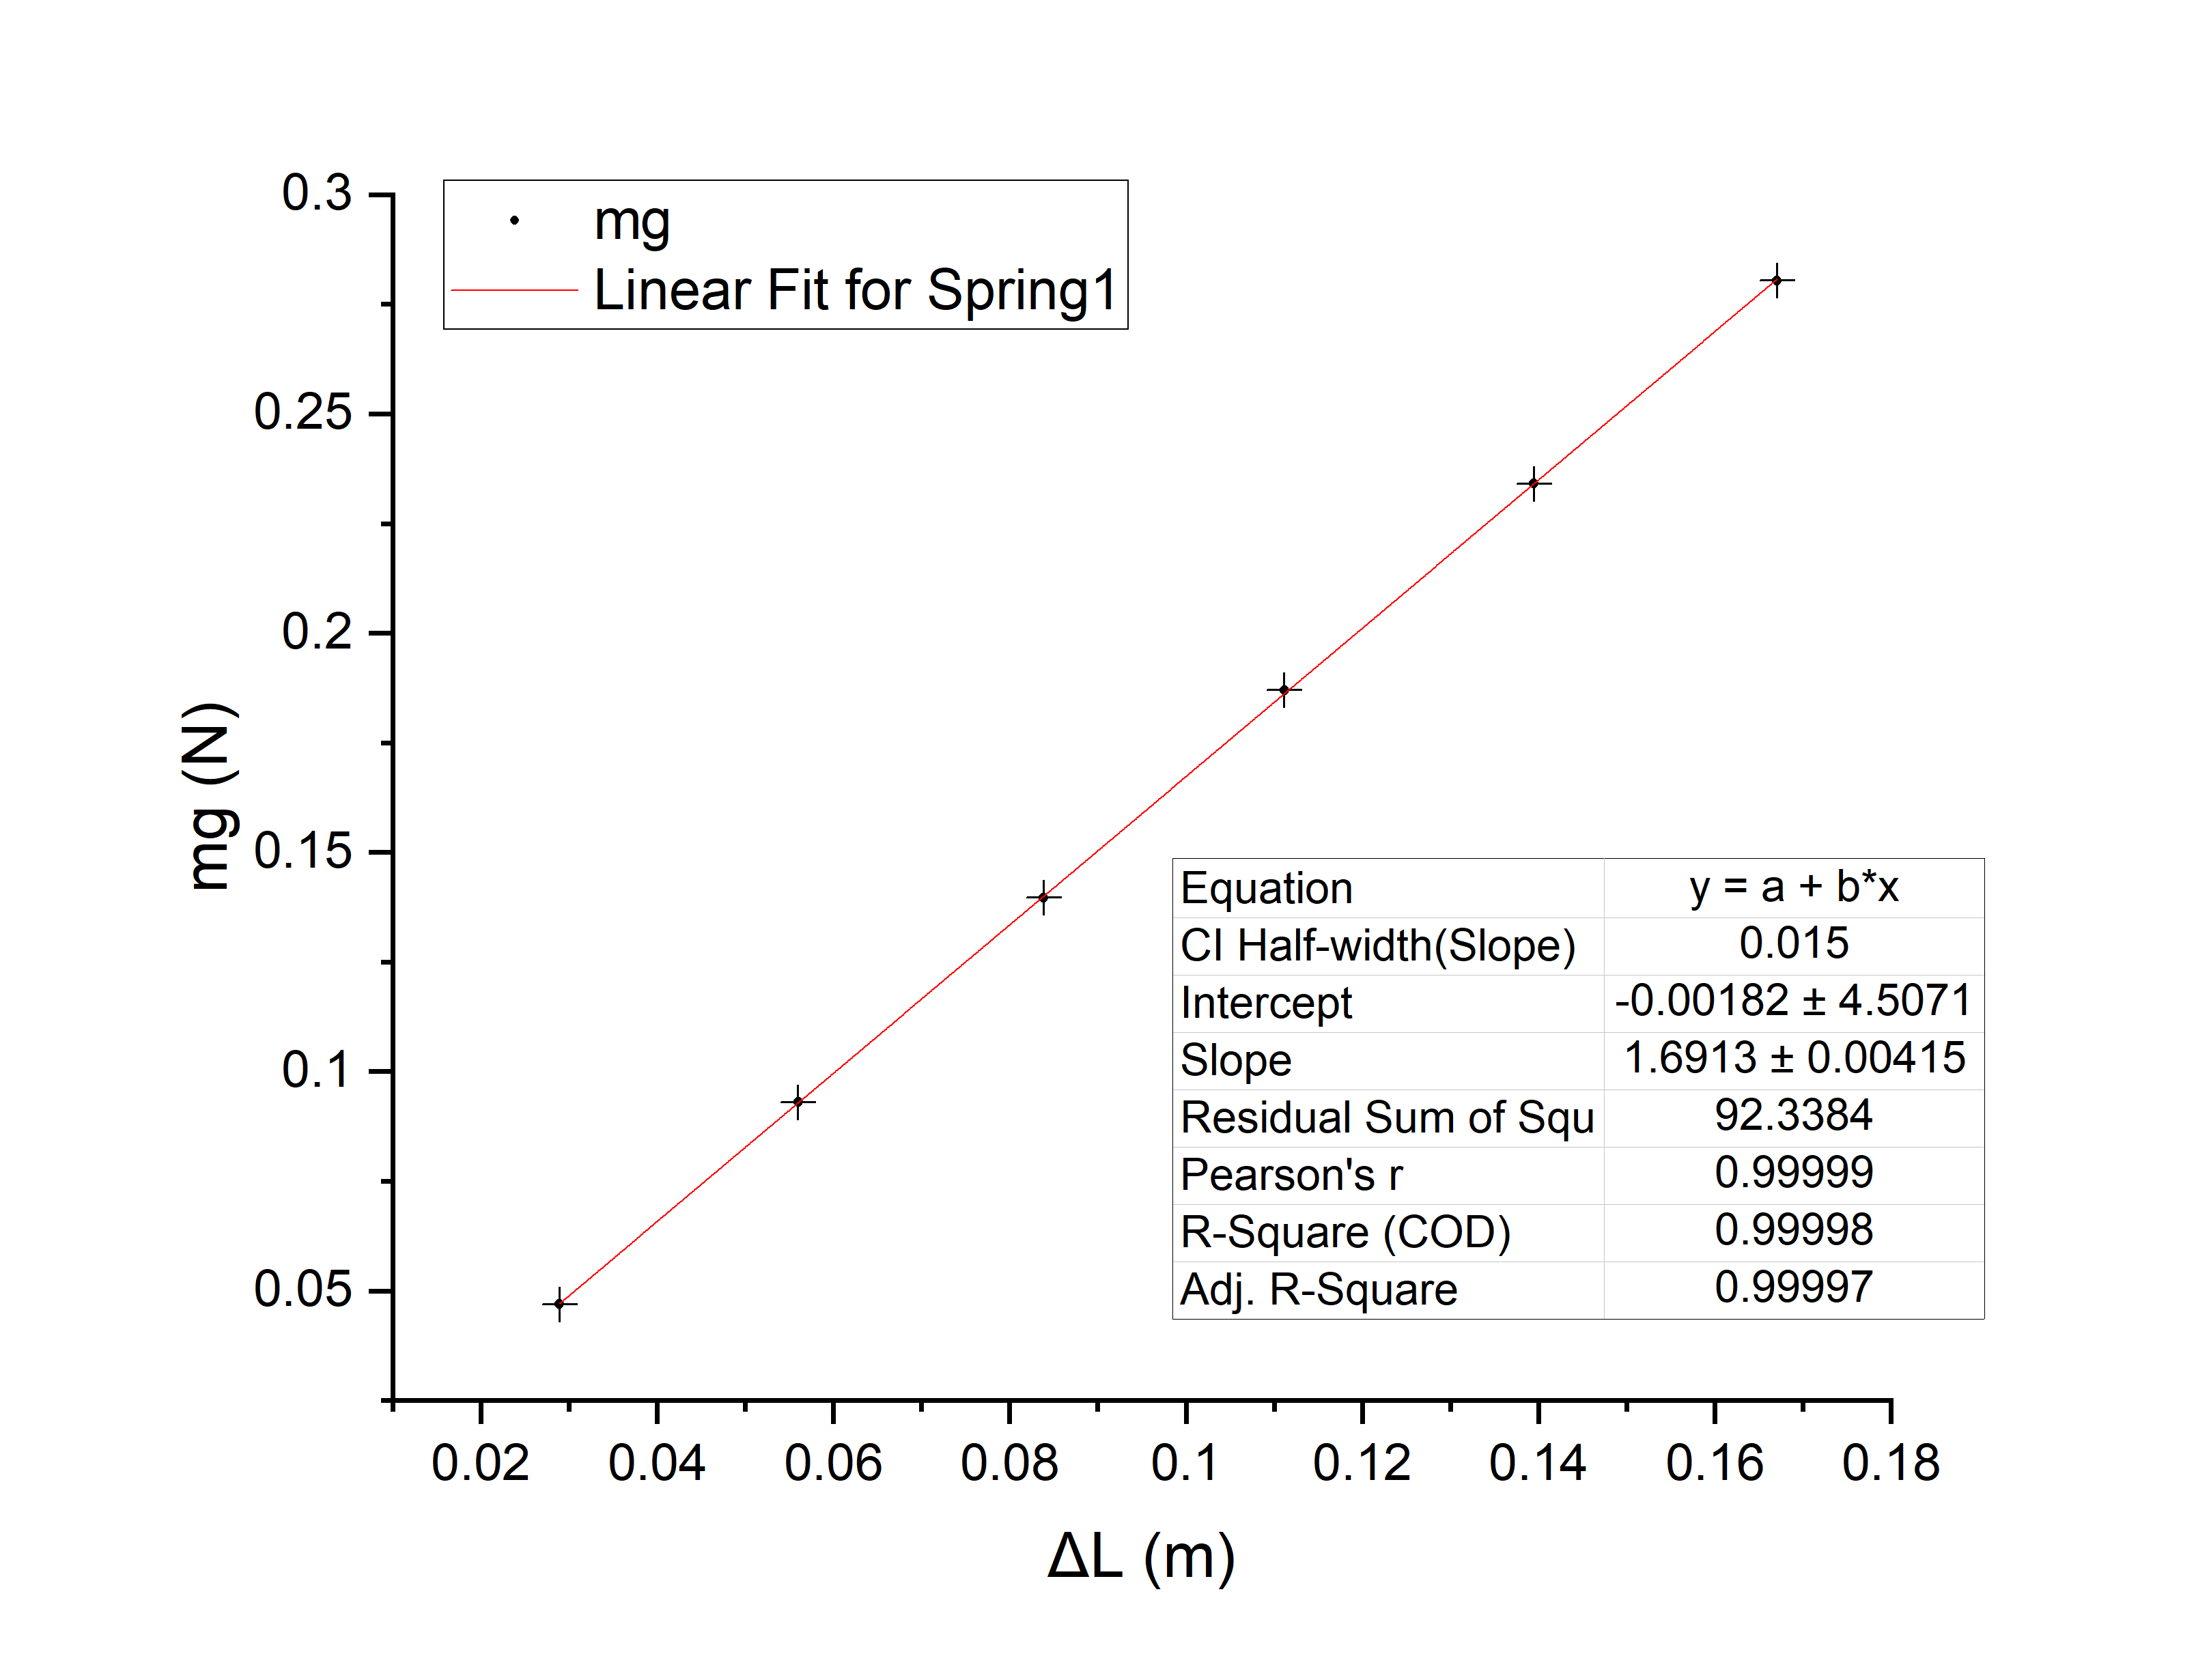
\includegraphics[scale=0.35]{k1.png}
    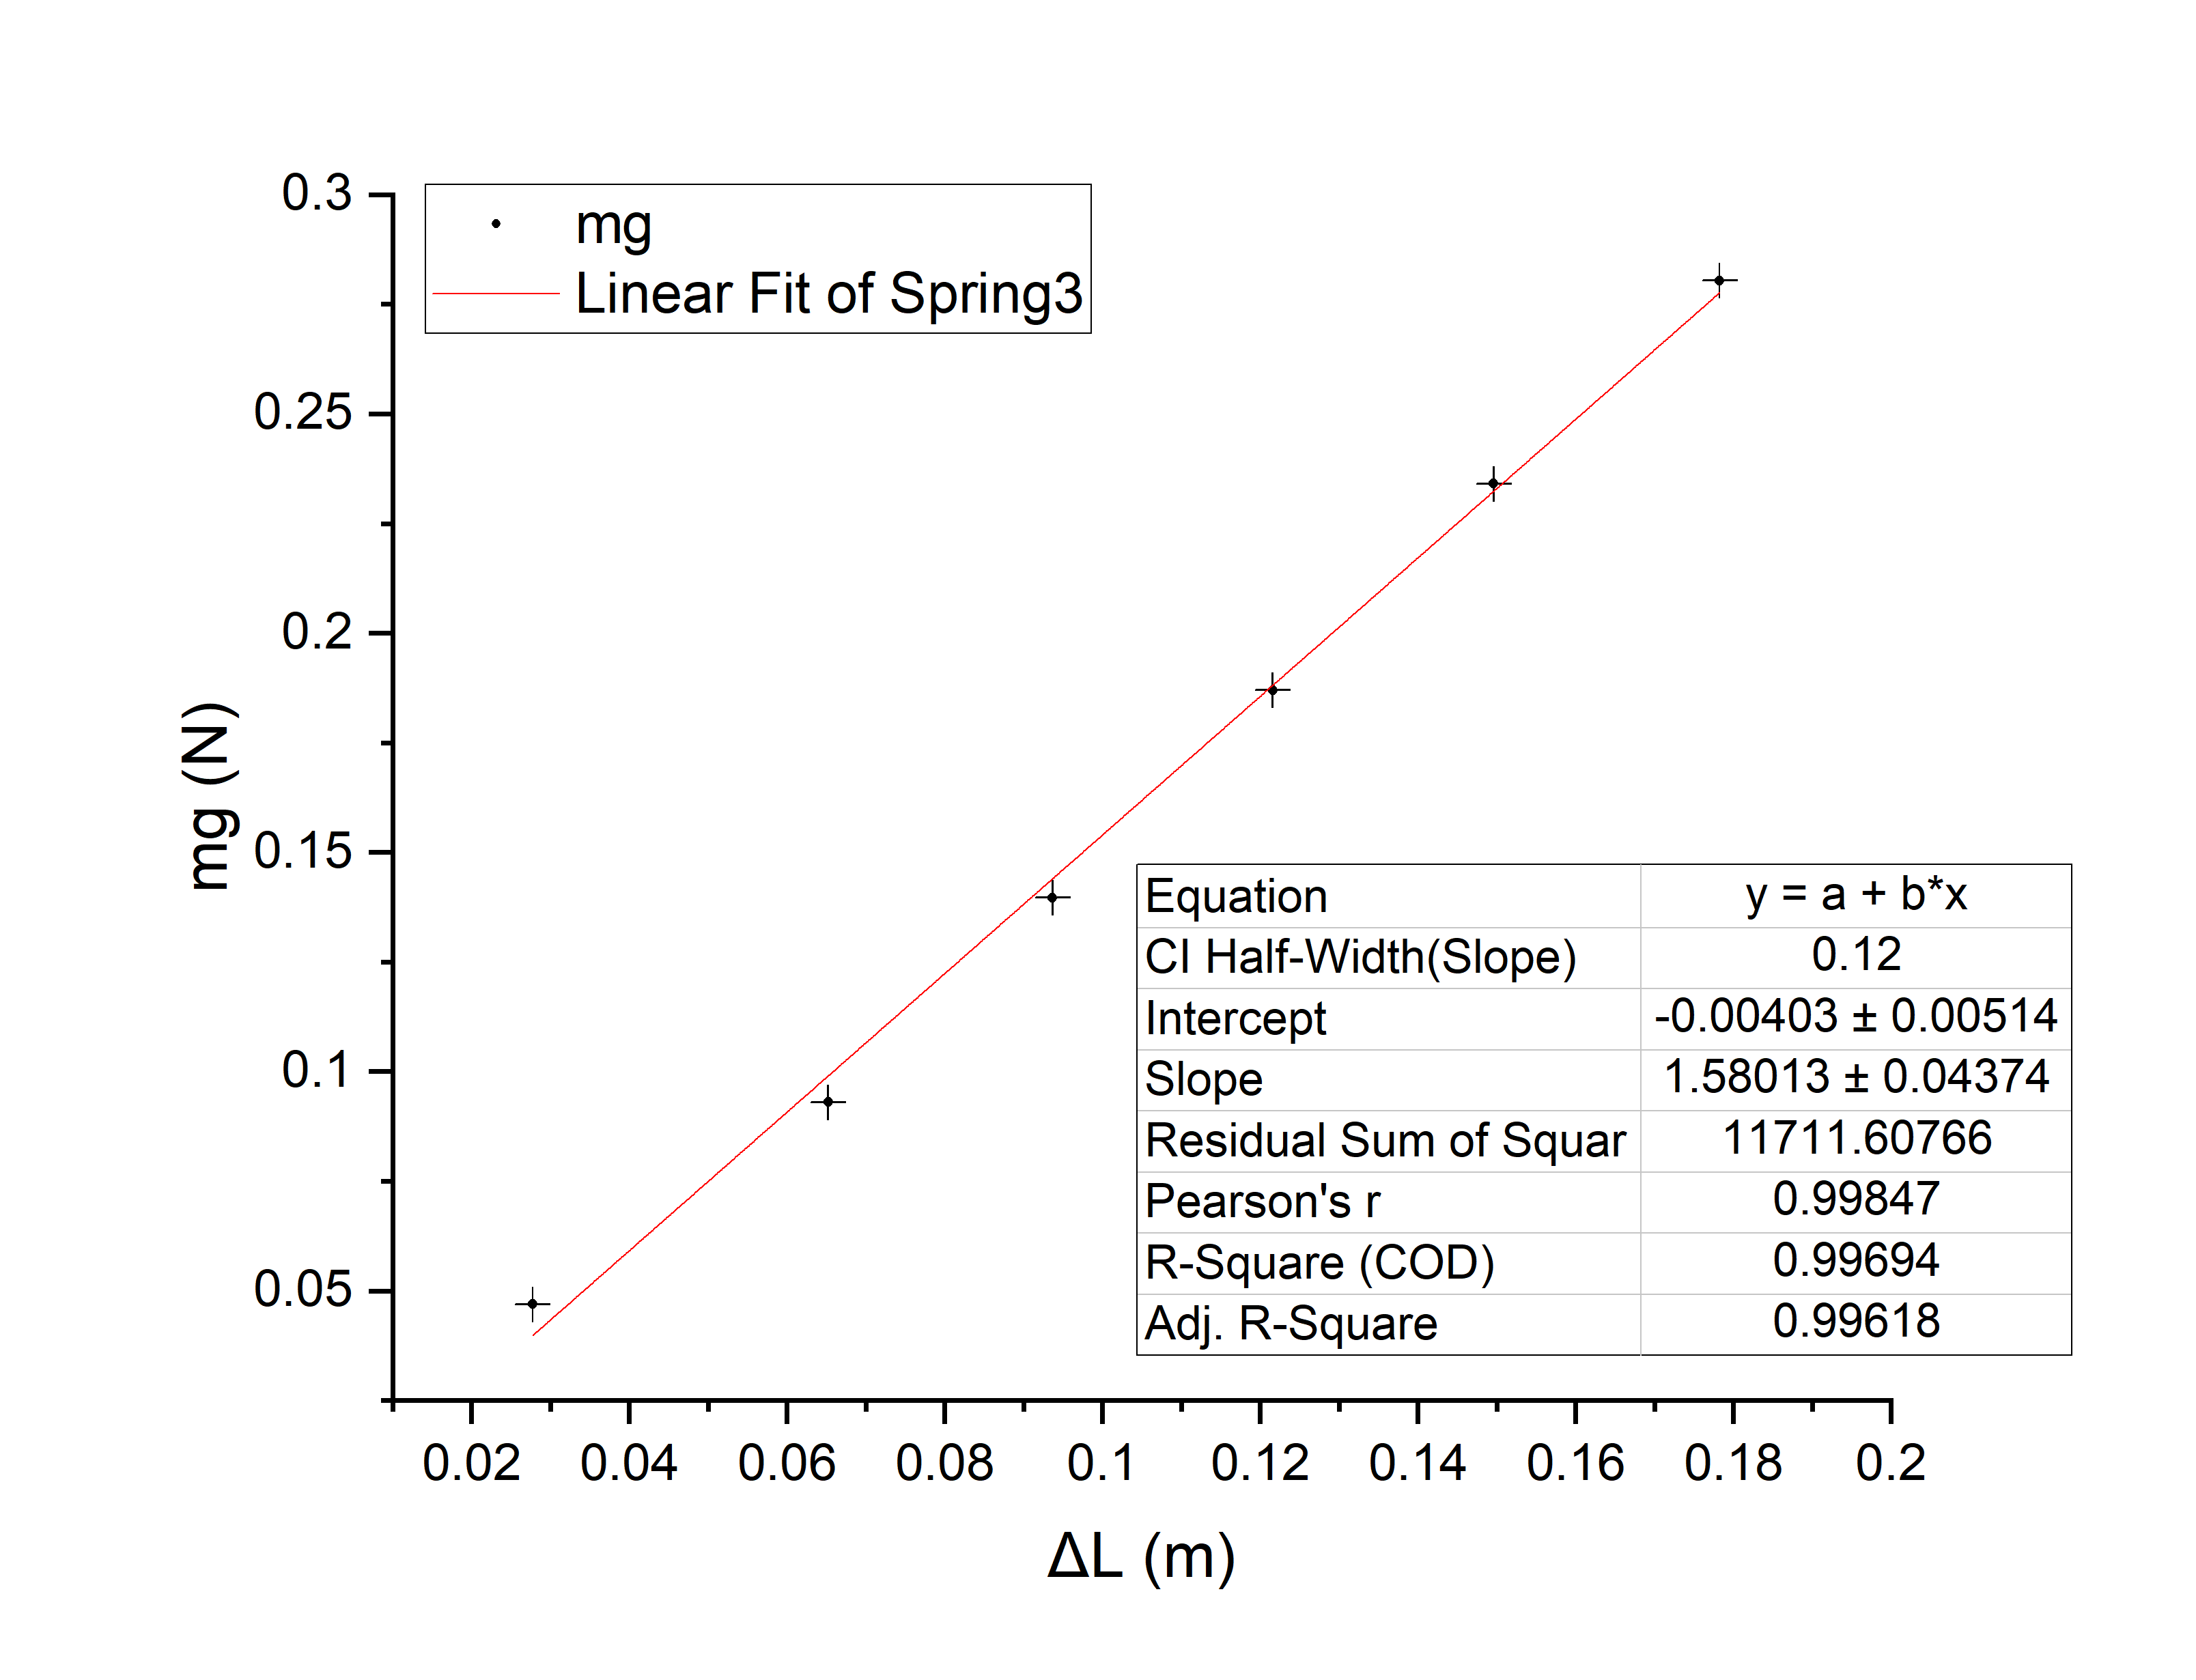
\includegraphics[scale=0.35]{k2.png}
    \caption{The linear fit figures of spring 1, 2}
    \end{figure}
\end{center}


%----------------------------------------------------------------------------------------
%	SECTION 7
%----------------------------------------------------------------------------------------
\section{Reference}
Qin Tian, Zheng Huan, Li Yingyu, Li Tiantian, Mateusz Krzyzosiak, Vp141, Exercise 3, Simple Harmonic Motion:
Oscillations in Mechanical Systems

%----------------------------------------------------------------------------------------
%	DATASHEET
%----------------------------------------------------------------------------------------

\newpage
{\LARGE\textbf{APPENDIX}}
\setcounter{section}{0}
\renewcommand\thesection{\Alph{section}}

\section{A Uncertainty Analysis}
\section{Uncertainty in Measurement of Spring Constant}
\subsection{Uncertainty of the weight measurement}
$$w=mg$$
$$\frac{\partial_w}{\partial_m}=g=9.794m/s^2$$
$$\frac{\partial_v}{\partial_g}=m$$
$$u_m=\Delta_A=0.01g$$
$$u_g=0$$
$$u_w=\sqrt{(\frac{\partial_w}{\partial_m})^2{u_m}^2+(\frac{\partial_w}{\partial_g})^2{u_g}^2}=\sqrt{(9.794)^2\times0.00001^2+m^2 \times 0^2}=0.00001N$$
\subsection{Uncertainty of the spring deformation measurement}
$$\Delta L=L-L0$$
According to the uncertainty propagation formula,
$$u_{\Delta L}=\sqrt{{u_L}^2\times 2}=\sqrt{0.00002^2\times 2}=0.00003m$$
\subsection{Uncertainty of k}
Through the help of origin